\documentclass[12pt]{article}
\usepackage{hyperref,amsmath,amsfonts,fullpage,color}
\usepackage{enumitem}
\usepackage{tikz}
\usetikzlibrary{arrows.meta}
\newcommand{\be}{\begin{equation}}
\newcommand{\ee}{\end{equation}}
\newcommand{\bh}{\bar{h}}
\newcounter{ansno}
\newcommand{\ans}[1]{\vspace{2em}\stepcounter{ansno}
\noindent{\bf Question \theansno.} \emph{(#1)}\\[0.5em]
}
\begin{document}

\begin{center}
{\bf\Large General Relativity}\\[0.5em]
{\bf\large Final Examination --- Answers}
\end{center}
\vspace{1em}
\hrule

% ---------------------------------------------------------------
\ans{2 points}
\textbf{Transformation of the Riemann tensor.} Under $x^\mu \to x'^\mu(x)$,
\be
R'^\mu{}_{\nu\rho\sigma} = \frac{\partial x'^\mu}{\partial x^\alpha}\,
\frac{\partial x^\beta}{\partial x'^\nu}\,
\frac{\partial x^\gamma}{\partial x'^\rho}\,
\frac{\partial x^\delta}{\partial x'^\sigma}\,
R^\alpha{}_{\beta\gamma\delta}.
\ee
That is, one upper index picks up a factor $\partial x'/\partial x$ and each of the three lower indices picks up a factor $\partial x/\partial x'$.

\textbf{Ricci tensor.} Define $R_{\mu\nu} = R^\rho{}_{\mu\rho\nu}$. Applying the transformation law with the contracted index $\rho$:
\begin{align*}
R'_{\mu\nu} = R'^\rho{}_{\mu\rho\nu}
&= \frac{\partial x'^\rho}{\partial x^\alpha}\,
\frac{\partial x^\beta}{\partial x'^\mu}\,
\frac{\partial x^\gamma}{\partial x'^\rho}\,
\frac{\partial x^\delta}{\partial x'^\nu}\,
R^\alpha{}_{\beta\gamma\delta} \\
&= \frac{\partial x^\beta}{\partial x'^\mu}\,
\frac{\partial x^\delta}{\partial x'^\nu}\,
\left(\frac{\partial x'^\rho}{\partial x^\alpha}\frac{\partial x^\gamma}{\partial x'^\rho}\right)
R^\alpha{}_{\beta\gamma\delta}.
\end{align*}
The bracket is $\frac{\partial x^\gamma}{\partial x^\alpha}=\delta^\gamma_\alpha$ (chain rule), so
\begin{align*}
R'_{\mu\nu} &= \frac{\partial x^\beta}{\partial x'^\mu}\,
\frac{\partial x^\delta}{\partial x'^\nu}\, \delta^\gamma_\alpha\, R^\alpha{}_{\beta\gamma\delta}
= \frac{\partial x^\beta}{\partial x'^\mu}\,
\frac{\partial x^\delta}{\partial x'^\nu}\, R^\gamma{}_{\beta\gamma\delta}
= \frac{\partial x^\beta}{\partial x'^\mu}\,
\frac{\partial x^\delta}{\partial x'^\nu}\, R_{\beta\delta}.
\end{align*}
This is precisely the transformation law of a $(0,2)$ tensor, so $R_{\mu\nu}$ is a tensor. The key step is that the contraction removes the one upper index and one lower index that transform inversely, leaving a covariant tensor.

% ---------------------------------------------------------------
\ans{3a: 2 points; 3b: 1 point}
Convention: $\nabla_\mu V^\rho = \partial_\mu V^\rho + \hat\Gamma_{\mu\nu}{}^\rho V^\nu$ (the sign and index ordering do not change the conclusions below). Write $\hat\Gamma_{\mu\nu}{}^\rho = \Gamma_{\mu\nu}{}^\rho + K_{\mu\nu}{}^\rho$ with
\be
K_{\mu\nu}{}^\rho = \frac{1}{12} g^{\rho\sigma} H_{\mu\nu\sigma}.
\ee
Lowering the last index, $K_{\mu\nu\rho} \equiv K_{\mu\nu}{}^\sigma g_{\sigma\rho} = \frac{1}{12}H_{\mu\nu\rho}$.

\textbf{(a) Torsion.} The torsion tensor is $T^\rho{}_{\mu\nu} = \hat\Gamma_{\mu\nu}{}^\rho - \hat\Gamma_{\nu\mu}{}^\rho$. The Levi-Civita part is symmetric, so only $K$ contributes:
\begin{align*}
T^\rho{}_{\mu\nu} &= K_{\mu\nu}{}^\rho - K_{\nu\mu}{}^\rho
= \frac{1}{12} g^{\rho\sigma}\left(H_{\mu\nu\sigma} - H_{\nu\mu\sigma}\right)
= \frac{1}{12} g^{\rho\sigma}\cdot 2H_{\mu\nu\sigma}
= \frac{1}{6} H^\rho{}_{\mu\nu},
\end{align*}
where we used $H_{\nu\mu\sigma} = -H_{\mu\nu\sigma}$ (total antisymmetry). Since $H\neq 0$ in general, \textbf{the connection is not torsion-free}. (The torsion is totally antisymmetric, which is the usual situation for string-frame connections with a $B$-field.)

\textbf{Metric compatibility.} Require $\hat\nabla_\mu g_{\nu\rho}=0$. Using the Levi-Civita connection is already metric compatible, so only the $K$ terms remain:
\begin{align*}
\hat\nabla_\mu g_{\nu\rho}
&= \partial_\mu g_{\nu\rho} - \hat\Gamma_{\mu\nu}{}^\sigma g_{\sigma\rho} - \hat\Gamma_{\mu\rho}{}^\sigma g_{\nu\sigma} \\
&= \underbrace{\left(\partial_\mu g_{\nu\rho} - \Gamma_{\mu\nu}{}^\sigma g_{\sigma\rho} - \Gamma_{\mu\rho}{}^\sigma g_{\nu\sigma}\right)}_{=\,\nabla_\mu g_{\nu\rho}=0} - K_{\mu\nu\rho} - K_{\mu\rho\nu} \\
&= -\frac{1}{12}\left(H_{\mu\nu\rho} + H_{\mu\rho\nu}\right) = 0,
\end{align*}
because $H_{\mu\rho\nu} = -H_{\mu\nu\rho}$. Hence \textbf{the connection is metric compatible}, even though it has torsion. (This is a metric-compatible connection with totally antisymmetric torsion.)

\textbf{Answer to (a):} not torsion-free; yes, metric compatible.

\textbf{(b) Geodesics.} A geodesic satisfies
\be
\frac{d^2 x^\mu}{d\lambda^2} + \hat\Gamma_{\nu\rho}{}^\mu \frac{dx^\nu}{d\lambda}\frac{dx^\rho}{d\lambda} = 0.
\ee
The difference from the Levi-Civita geodesic equation is
\be
K_{\nu\rho}{}^\mu \dot x^\nu \dot x^\rho = \frac{1}{12} g^{\mu\sigma} H_{\nu\rho\sigma}\, \dot x^\nu \dot x^\rho.
\ee
The tangent vector contraction $\dot x^\nu \dot x^\rho$ is symmetric in $(\nu,\rho)$, while $H_{\nu\rho\sigma}$ is antisymmetric in $(\nu,\rho)$. A symmetric tensor contracted with an antisymmetric one vanishes:
\be
H_{\nu\rho\sigma}\,\dot x^\nu \dot x^\rho = \tfrac12 H_{\nu\rho\sigma}\left(\dot x^\nu \dot x^\rho + \dot x^\rho \dot x^\nu\right) = 0 \quad\text{(since } H_{\nu\rho\sigma} = -H_{\rho\nu\sigma}\text{)}.
\ee
Therefore the geodesic equations of $\hat\Gamma$ and of the Levi-Civita connection coincide, so the geodesics are the same. (Affine parametrisation is preserved too, since the same equation is satisfied with the same $\lambda$.)

% ---------------------------------------------------------------
\ans{4a: 2 points; 4b: 2 points}
\textbf{(a) Singularities.} The metric components are singular where $f(r)=0$ or $r=0$:
\begin{itemize}
\item $r = 2GM$ (the Schwarzschild radius): $g_{tt}=-f\to 0$ and $g_{rr}=f^{-1}\to\infty$. This is a \emph{coordinate} singularity: it is an artefact of the Schwarzschild $(t,r)$ chart. Curvature invariants are finite there. For example, the Kretschmann scalar is
\be
R_{\mu\nu\rho\sigma}R^{\mu\nu\rho\sigma} = \frac{48 G^2M^2}{r^6},
\ee
which is finite at $r=2GM$: $K(2GM) = \dfrac{48G^2M^2}{(2GM)^6} = \dfrac{3}{4G^4M^4}$. So a freely falling observer crosses $r=2GM$ without feeling anything special; it is a one-way horizon.
\item $r = 0$: here $K = 48G^2M^2/r^6 \to \infty$ and the curvature diverges. This is a \emph{genuine} (physical) curvature singularity, which cannot be removed by any choice of coordinates.
\end{itemize}
\textbf{Answer:} you should be concerned only about $r=0$. Once inside $r<2GM$ the coordinate $r$ becomes timelike, so $r$ decreases monotonically for any future-directed worldline. You cannot avoid reaching $r=0$, and there the tidal forces diverge (spaghettification). Crossing $r=2GM$ itself is not dangerous in the sense of local curvature; your friends' worry is about the physical singularity at $r=0$, which lies in your future, not about the horizon.

\textbf{(b) Ingoing Eddington--Finkelstein coordinates.} Let $r_* = r + 2GM\ln\left|\frac{r}{2GM}-1\right|$. Then
\be
\frac{dr_*}{dr} = 1 + 2GM\cdot\frac{1}{r-2GM} = \frac{r}{r-2GM} = \frac{1}{f(r)},
\ee
so $v = t + r_*$ gives $dv = dt + dr/f$, i.e. $dt = dv - dr/f$. Substituting into the Schwarzschild metric:
\begin{align*}
ds^2 &= -f\,dt^2 + \frac{dr^2}{f} + r^2 d\Omega^2 \\
&= -f\left(dv - \frac{dr}{f}\right)^2 + \frac{dr^2}{f} + r^2 d\Omega^2 \\
&= -f\,dv^2 + 2\,dv\,dr - \frac{dr^2}{f} + \frac{dr^2}{f} + r^2 d\Omega^2 \\
&= -f(r)\,dv^2 + 2\,dv\,dr + r^2\left(d\theta^2 + \sin^2\theta\, d\phi^2\right).
\end{align*}
Thus
\be
ds^2 = -\left(1-\frac{2GM}{r}\right)dv^2 + 2\,dv\,dr + r^2\left(d\theta^2+\sin^2\theta\,d\phi^2\right),
\ee
and all components are finite and smooth at $r=2GM$. The determinant is $-r^4\sin^2\theta$, which is nonzero for $r>0$, so $(v,r,\theta,\phi)$ is a valid chart across the horizon.

\textbf{Connection to (a).} The singularity at $r=2GM$ disappears in these coordinates, confirming it is a coordinate artefact. Ingoing null rays are $v=\text{const}$ and cross $r=2GM$ smoothly. The only remaining singularity is at $r=0$, where the curvature (and the $1/r^6$ Kretschmann scalar) genuinely diverges. An infalling observer therefore crosses the horizon safely and meets the true singularity at $r=0$ in finite proper time.

% ---------------------------------------------------------------
\ans{5a: 2 points; 5b: 1 point; 5c: 2 points}
\textbf{(a)} The metric is of Friedmann--Lema\^itre--Robertson--Walker form,
\be
ds^2 = -dt^2 + a(t)^2\,d\Sigma_3^2,\qquad d\Sigma_3^2 = d\chi^2 + \sin^2\chi\left(d\theta^2+\sin^2\theta\,d\phi^2\right),
\ee
with the scale factor
\be
a(t) = L\cosh(t/L).
\ee
It is homogeneous and isotropic on spatial slices, which matches the cosmological principle that describes our universe at large scales. It is a candidate for our universe because: (i) it describes a universe with a positive cosmological constant, $\Lambda = 3/L^2$, so that the expansion accelerates at late times, consistent with the observed accelerating expansion (dark energy); and (ii) at late times $a \approx \tfrac{L}{2}e^{t/L}$, i.e. an exponential expansion with Hubble parameter $H = 1/L$, which is approximately the behaviour of our universe in the far future. Caveat: this closed slicing has spatial curvature $k=+1$, whereas observations indicate nearly flat space; the same de Sitter spacetime can be sliced with flat sections, $a=e^{t/L}$, which is the more realistic description.

\textbf{(b)} Let $g_{\mu\nu} = \Omega^2\bar g_{\mu\nu}$ with $\Omega$ a positive, smooth function. Causal structure is determined by which curves are timelike, null, or spacelike:
\begin{itemize}
\item A curve is null for $g$ iff $g_{\mu\nu}\dot x^\mu\dot x^\nu = \Omega^2\,\bar g_{\mu\nu}\dot x^\mu\dot x^\nu = 0$, iff $\bar g_{\mu\nu}\dot x^\mu\dot x^\nu=0$ (since $\Omega^2\neq 0$). So null curves of $g$ and $\bar g$ coincide.
\item Similarly the sign of $g_{\mu\nu}\dot x^\mu\dot x^\nu$ equals the sign of $\bar g_{\mu\nu}\dot x^\mu\dot x^\nu$, so timelike and spacelike curves are also preserved.
\end{itemize}
Hence the light cones (the null directions at each point) are the same, and any two points joined by a causal curve in one metric are joined by one in the other. Thus the causal structure, and hence a Penrose diagram, is identical, even though distances and geodesics may differ. Angles are also preserved (conformal invariance).

\textbf{(c)} Set $\cosh(t/L) = \sec\eta$ with $-\pi/2<\eta<\pi/2$.

\emph{Time coordinate.} Differentiate: $\frac{1}{L}\sinh(t/L)\,dt = \sec\eta\tan\eta\,d\eta$. Since $\sinh(t/L) = \sqrt{\cosh^2(t/L)-1} = \sqrt{\sec^2\eta-1} = |\tan\eta|$, and $t$ and $\eta$ have the same sign (take $t>0 \leftrightarrow 0<\eta<\pi/2$, the other half follows by symmetry), we have $\sinh(t/L)=\tan\eta$, so
\be
dt = L\sec\eta\, d\eta.
\ee

\emph{Metric.} Then
\begin{align*}
-dt^2 &= -L^2\sec^2\eta\, d\eta^2, \\
a^2 &= L^2\cosh^2(t/L) = L^2\sec^2\eta,
\end{align*}
so
\be
ds^2 = L^2\sec^2\eta\left(-d\eta^2 + d\chi^2 + \sin^2\chi\left(d\theta^2+\sin^2\theta\,d\phi^2\right)\right).
\ee
That is, $g_{\mu\nu} = \Omega^2\bar g_{\mu\nu}$ with $\Omega = L\sec\eta$ and
\be
\bar g = -d\eta^2 + d\chi^2 + \sin^2\chi\, d\Omega_2^2 ,
\ee
which is the Einstein static universe $\mathbb{R}\times S^3$ (with $\chi\in(0,\pi)$). Since $\Omega$ is finite for $|\eta|<\pi/2$ and diverges at $\eta=\pm\pi/2$, the surfaces $\eta=\pm\pi/2$ are at conformal infinity, $\mathcal{I}^\pm$, while $\eta=0$ is the $t=0$ slice (the minimum of $a$, the ``throat'').

\emph{Penrose diagram.} Use coordinates $(\eta,\chi)$ with $\theta,\phi$ suppressed (each point of the diagram is a 2-sphere of radius $L\sec\eta\sin\chi$). The diagram is the square $-\pi/2<\eta<\pi/2$, $0<\chi<\pi$, with:
\begin{itemize}
\item the top edge $\eta=\pi/2$ = future infinity $\mathcal{I}^+$ and the bottom edge $\eta=-\pi/2$ = past infinity $\mathcal{I}^-$ (both spacelike);
\item the left and right edges $\chi=0$ and $\chi=\pi$, which are the worldlines of the north and south poles of the 3-sphere (timelike; regular, not boundaries);
\item the 45$^\circ$ diagonals, which are null geodesics (light rays), since $\bar g$ is conformally related and $d\chi=\pm d\eta$.
\end{itemize}

\begin{center}
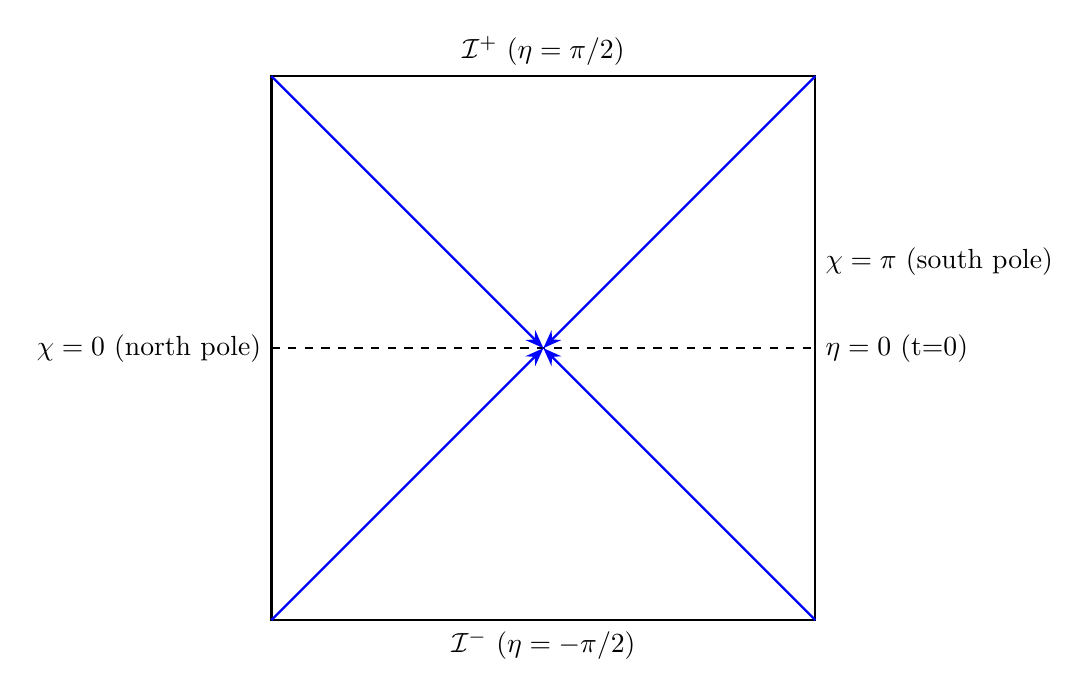
\begin{tikzpicture}[scale=2.2, >=Stealth, thick]
  % square: x = chi in (0,pi) mapped to [0,pi], y = eta in (-pi/2,pi/2)
  \draw[thick] (0,-1.57) rectangle (3.14,1.57);
  \draw[dashed] (0,0) -- (3.14,0) node[right] {$\eta=0$ (t=0)};
  % null rays from the south-pole worldline? draw light-cone diagonals
  \draw[->, blue] (0,-1.57) -- (1.57,0);
  \draw[->, blue] (3.14,-1.57) -- (1.57,0);
  \draw[->, blue] (0,1.57) -- (1.57,0);
  \draw[->, blue] (3.14,1.57) -- (1.57,0);
  \node[above] at (1.57,1.57) {$\mathcal{I}^+$ ($\eta=\pi/2$)};
  \node[below] at (1.57,-1.57) {$\mathcal{I}^-$ ($\eta=-\pi/2$)};
  \node[left] at (0,0) {$\chi=0$ (north pole)};
  \node[right] at (3.14,0.5) {$\chi=\pi$ (south pole)};
  \node[below] at (0,-1.6) {};
\end{tikzpicture}
\end{center}
This is the standard de Sitter Penrose diagram: a square with the two spacelike infinities at top and bottom and the timelike pole worldlines as the vertical sides. Every point of the diagram is a 2-sphere (the pole lines are where the 2-spheres shrink to points). The diagram shows that the $\eta=0$ slice is the $t=0$ time-symmetric slice, and that light rays emitted from a pole worldline reach $\mathcal{I}^+$ along the diagonals.

% ---------------------------------------------------------------
\ans{6a: 1 point; 6b: 2 points; 6c: 3 points}
\textbf{(a) Gravitational waves from the gauge choice.} The gauge transformation $h_{\mu\nu}\to h_{\mu\nu}+\partial_\mu\xi_\nu+\partial_\nu\xi_\mu$ changes $\partial^\rho\bh_{\rho\nu}$ by $\Box\xi_\nu$. Since $\Box\xi_\nu$ can be set to anything, we can choose $\xi$ so that the \emph{harmonic (de Donder/Lorenz) gauge} holds:
\be
\partial^\rho \bh_{\mu\rho} = 0.
\ee
In this gauge, the symmetric derivative terms vanish:
\be
\partial^\rho\partial_{(\mu}\bh_{\nu)\rho} = \tfrac12\left(\partial_\mu\partial^\rho\bh_{\nu\rho} + \partial_\nu\partial^\rho\bh_{\mu\rho}\right) = 0,
\qquad
\partial^\rho\partial^\sigma\bh_{\rho\sigma} = 0.
\ee
The linearised equation then reduces to
\be
-\tfrac12\,\Box\bh_{\mu\nu} = 8\pi G T_{\mu\nu}
\quad\Longrightarrow\quad
\Box\bh_{\mu\nu} = -16\pi G\,T_{\mu\nu}.
\ee
In vacuum ($T_{\mu\nu}=0$) this is a wave equation $(-\partial_t^2+\nabla^2)\bh_{\mu\nu}=0$ with propagation speed $c=1$. Hence the metric perturbation propagates as waves: gravitational waves. Further imposing transverse-traceless conditions leaves only two independent polarisations (the $+$ and $\times$ modes), as in part b).

\textbf{(b) Proper distance.} The perturbation is $h_{\mu\nu}$ as given, with $\eta_{\mu\nu} = \mathrm{diag}(-1,1,1,1)$. The metric is $g_{\mu\nu} = \eta_{\mu\nu} + h_{\mu\nu}$. The given $h$ is transverse and traceless: $\partial^\mu h_{\mu\nu}=0$ and $\eta^{\mu\nu}h_{\mu\nu} = -0 + h_+ - h_+ + 0 = 0$. The test particles are freely falling, so their coordinates remain constant: $\Gamma^i{}_{tt} = \tfrac12(2\partial_t h_{it} - \partial_i h_{tt}) = 0$ and $\Gamma^i{}_{jk}=0$ at this order for $h_{ij}$ depending only on $t-z$ and evaluated at the particles.

Proper distance is measured along a spatial path at fixed $t$ (simultaneous events). The line element along the $x$-axis ($y=z=0$) at fixed $t$ is
\begin{align*}
ds^2 &= g_{xx}\,dx^2 = \left(1 + h_{xx}\right)dx^2 = \left(1 + h_+(t-z)\right)dx^2 \\
&\text{so at } z=0:\quad ds^2 = \left(1+h_+(t)\right)dx^2.
\end{align*}
Integrating from $x=0$ to $x=L_x$:
\be
\Delta s = \int_0^{L_x}\sqrt{1+h_+(t)}\,dx = L_x\sqrt{1+h_+(t)} \approx L_x\left(1+\tfrac12 h_+(t)\right),
\ee
using $\sqrt{1+\epsilon}\approx 1+\epsilon/2$ for $|h_+|\ll 1$. (The approximation $h_+(t-z)\approx h_+(t)$ holds across the arm because the wave varies on a timescale much longer than $L_x/c$.)

For the third particle at $(0,L_y,0)$, the relevant component is $h_{yy} = -h_+$, so
\be
ds^2 = (1 - h_+(t))\,dy^2 \quad\Longrightarrow\quad \Delta s = L_y\sqrt{1-h_+(t)} \approx L_y\left(1-\tfrac12 h_+(t)\right).
\ee

\textbf{(c) Binary inspiral, merger, ringdown.}
\begin{itemize}
\item \textbf{Inspiral.} The two bodies orbit each other and accelerate, so the system radiates gravitational waves (quadrupole radiation). The energy and angular momentum carried away make the orbit shrink: the separation decreases and the orbital angular frequency increases. For circular orbits at leading (quadrupole) order, the orbital frequency increases as the separation shrinks ($\Omega^2 r^3 = G M_{\rm tot}$, so $\Omega\propto r^{-3/2}$ and $\dot f\propto \mathcal{M}^{5/3}f^{11/3}$). The GW frequency is $f_{\rm GW}=2f_{\rm orb}$, so the observed signal is a chirp, with both frequency and amplitude increasing.
\item \textbf{Merger.} When the separation becomes comparable to the Schwarzschild radius of the system, the bodies plunge together. The motion is highly nonlinear, the signal peaks in frequency and amplitude, and the strongest emission occurs.
\item \textbf{Ringdown.} The remnant black hole settles into a stationary Kerr state by emitting quasinormal modes, which damp exponentially: $h(t)\propto e^{-t/\tau}\cos(\omega t+\phi)$.
\end{itemize}
\textbf{Detection by an interferometer.} A Michelson interferometer has two perpendicular arms, along $x$ and $y$. A passing wave changes the arm lengths according to the proper-distance result in (b): the $x$-arm changes by $\delta L_x = \tfrac12 h_+ L_x$ and the $y$-arm by $\delta L_y = -\tfrac12 h_+ L_y$. The changes are opposite, so the light round-trip times differ and the interference fringes shift. The output is proportional to $h_+(t)$ (the strain). For arms of length $L$, the differential arm change is $\delta L_{x}-\delta L_{y} = L h_+(t)$. The light's round-trip phase in each arm is $2\pi\cdot 2L/\lambda$, so the differential phase shift is
\be
\Delta\phi \approx \frac{2\pi}{\lambda}\cdot 2\,L\,h_+(t) = \frac{4\pi L}{\lambda}h_+(t),
\ee
which is small but measurable (large $L$ and a long optical path enhance it).

\textbf{Sketch of the signal.} The strain $h(t)$ as a function of time looks like:
\begin{center}
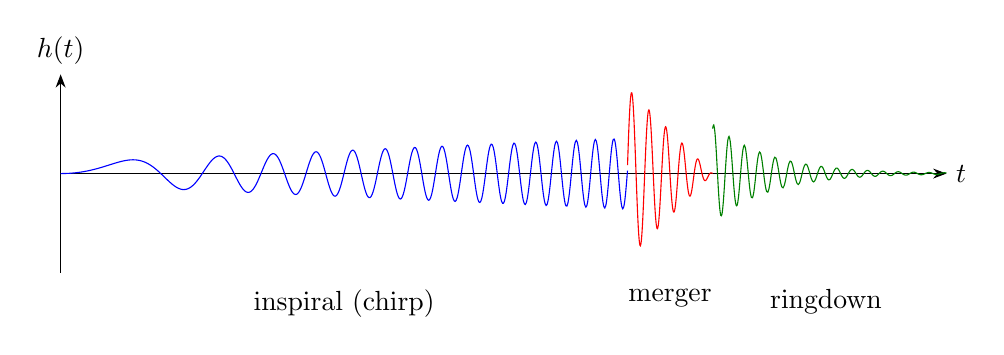
\begin{tikzpicture}[xscale=0.09, yscale=0.9, >=Stealth]
  % inspiral chirp: frequency and amplitude grow with time
  \draw[->] (0,0) -- (125,0) node[right] {$t$};
  \draw[->] (0,-1.4) -- (0,1.4) node[above] {$h(t)$};
  % inspiral: phase 360*k*x^2 gives frequency ~ x; amplitude grows
  \draw[domain=0:80, samples=600, smooth, variable=\x, blue]
    plot ({\x}, {(0.15+0.35*\x/80)*sin(360*0.0025*\x*\x)});
  % merger: largest amplitude, highest frequency
  \draw[domain=80:92, samples=200, smooth, variable=\x, red]
    plot ({\x}, {1.2*sin(360*0.0025*\x*\x)*(1-(\x-80)/12)});
  % ringdown: exponential damping at a fixed frequency
  \draw[domain=92:125, samples=200, smooth, variable=\x, green!50!black]
    plot ({\x}, {0.7*exp(-(\x-92)/8)*sin(360*0.0025*92*92 + 360*0.0025*2*92*(\x-92))});
  \node[below] at (40,-1.5) {inspiral (chirp)};
  \node[below] at (86,-1.5) {merger};
  \node[below] at (108,-1.5) {ringdown};
\end{tikzpicture}
\end{center}
(Schematic: frequency and amplitude increase during inspiral, peak at merger, then decay exponentially during ringdown.)

\textbf{Connection to the physics.} The chirp rate measures the chirp mass $\mathcal{M}=\frac{(m_1m_2)^{3/5}}{(m_1+m_2)^{1/5}}$, while the amplitude scales with distance and the chirp mass. The final ringdown frequency and damping time measure the properties (mass and spin) of the remnant black hole. The entire signal therefore encodes the binary's masses, orbit evolution, and final state.

\end{document}
